\documentclass{beamer}
\usepackage[english,russian]{babel}
\usepackage[utf8]{inputenc}
\usepackage{pagenumber}

\usepackage{hyperref}
% Стиль презентации
\usetheme[numbers, totalnumbers]{Dresden}
% цветовая схема
\usecolortheme{beaver}

\makeatletter
\defbeamertemplate*{footline}{Dresden}{
	\leavevmode%
	\hbox{%
	\begin{beamercolorbox}[wd=.3\paperwidth,ht=3.00ex,dp=1ex,center]{author in head/foot}%
		\usebeamerfont{author in head/foot}%
		\insertauthor	
	\end{beamercolorbox}%
	\begin{beamercolorbox}[wd=0.5\paperwidth,ht=3.00ex,dp=1ex,center]{title in head/foot}%
		\usebeamerfont{title in head/foot}\inserttitle
	\end{beamercolorbox}%
	\begin{beamercolorbox}[wd=.2\paperwidth,ht=3.00ex,dp=1ex,right]{date in head/foot}%
		\usebeamerfont{date in head/foot}\hspace*{2em}
		\insertframenumber{} / \inserttotalframenumber\hspace*{2ex}
	\end{beamercolorbox}}%
}
\makeatother

\begin{document}
\title{Оптимизация проверки задач для Linux* курсов}  
\author{Волков Д., Заславский М.}
\institute{Computer Science Center}
\date{\today} 

% -- Представление, приветы
\frame{\titlepage} 

% -- В рамках этого проекта я работал в основном над улучшением
% -- системы проверки вот этого курса на stepic, поднимите ваши
% -- руки, кто с этим курсом знаком (если кто-то поднял, то ещё
% -- поднимите кто прошел этот курс). Спросить, если ненулевые
% -- количества поднятых рук, долго ли приходилось ожидать про-
% -- верки задач.
\begin{frame}{Stepic}
	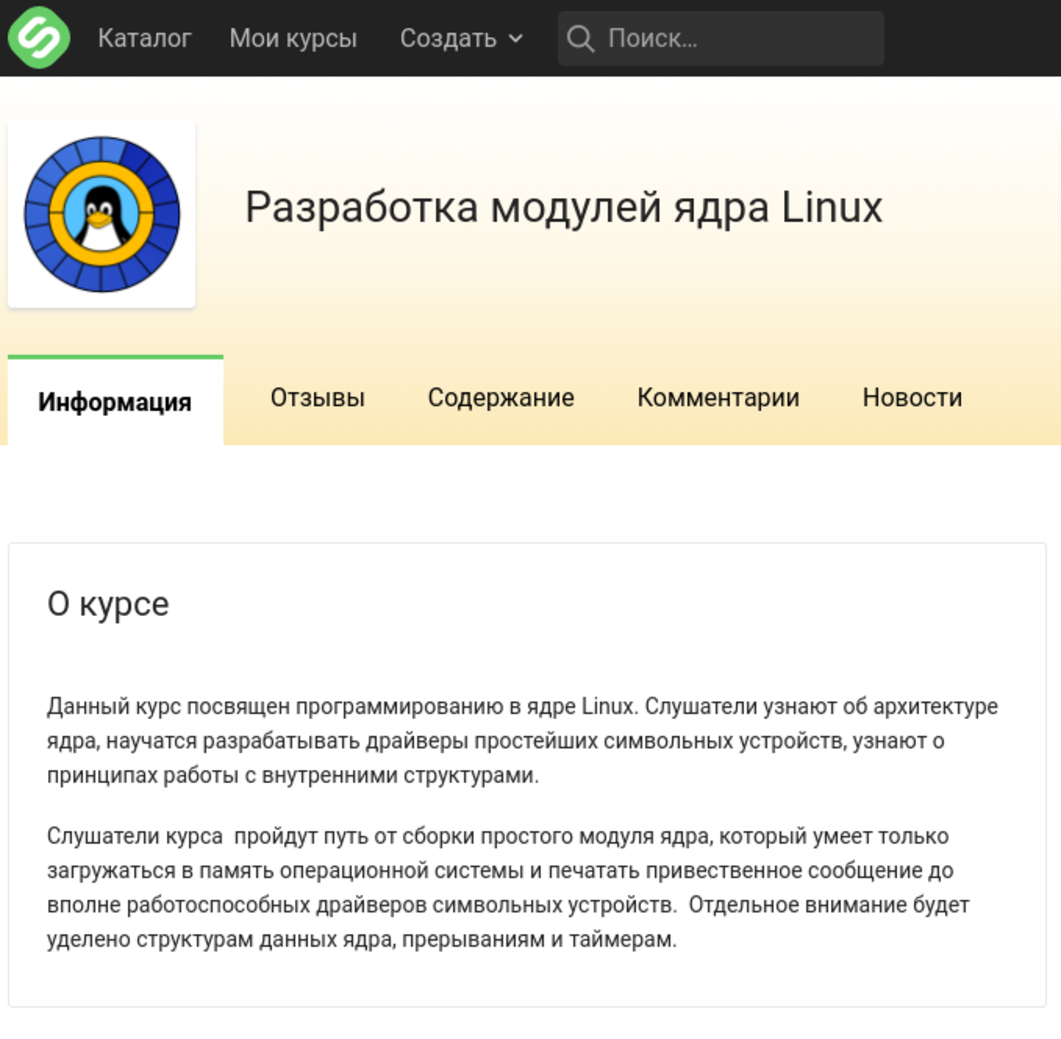
\includegraphics[width=100mm]{./stepic.pdf}
\end{frame}

% -- Спросить, есть ли тут кто-то, кто делал задачи для этого
% -- курса. 
% -- Работа над этим курсом породила некоторое количество про-
% -- блем.
\begin{frame}{Зачем?}
	\begin{itemize}
		\item Облегчить задачу составителям курсов
		\item Отделение проверяющей системы от тестов
		\item Сокращение времени ожидания вердикта пользователем
	\end{itemize}
\end{frame}

% -- Более формальный слайд, представляющий цели и задачи проекта.
% -- Каждая задача непосредственно вытекает из потребностей, сфор-
% -- мулированный выше.
\begin{frame}{Цели и задачи}
	\textbf{Цель проекта:} оптимизация структуры и производительности проверяющей системы.

	\textbf{Задачи:}
	\begin{itemize}
		\item Архитектурное разделение проверяющей системы и сценариев проверки отдельных заданий.
		\item Профилирование проверки решений
		\item Ускорение проверки решений 
	\end{itemize}
\end{frame}

% -- На слайде пример проблемы, связанной с взаимосвязью проверяющей системы
% -- и тестовых сценариев. 
\begin{frame}{На старте}
	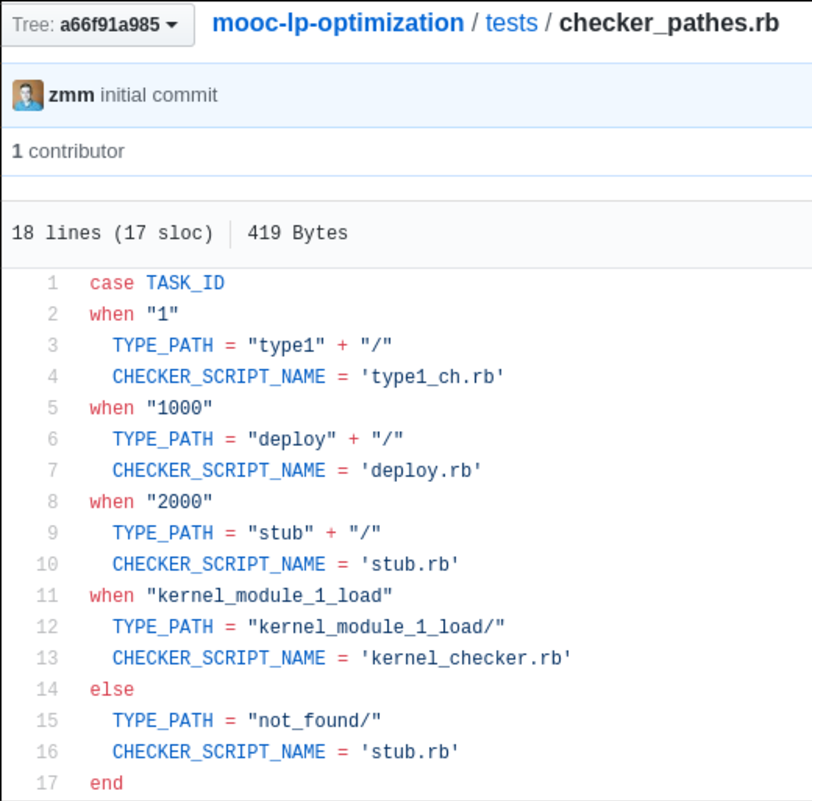
\includegraphics[width=80mm]{./patchesrb.pdf}
\end{frame}

% -- Здесь кусочек лога проверяющей системы. Особенности приведенных данных.
\begin{frame}{На старте}
	Виртуализация \textbf{KVM + Libvirt}
	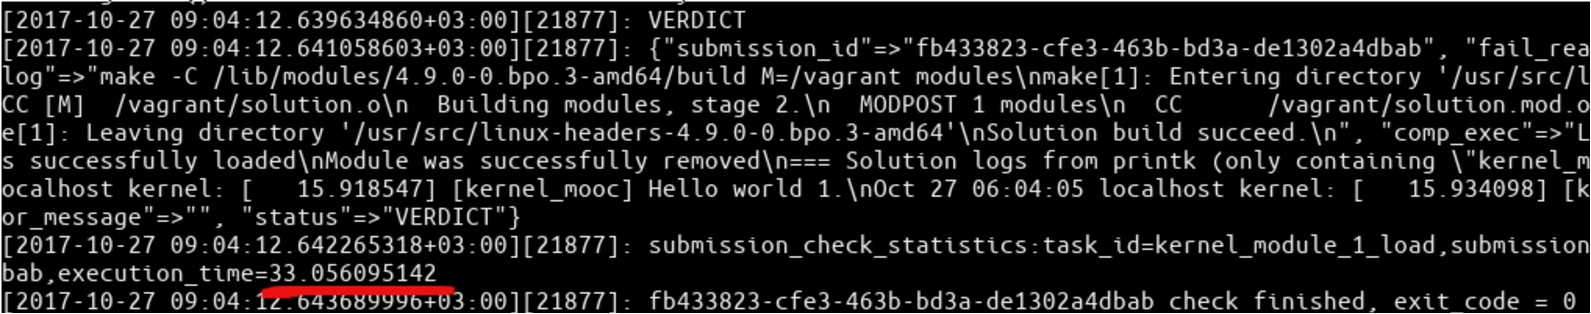
\includegraphics[width=115mm]{./length_start.pdf}
\end{frame}

% -- В рамках решения задачи о разделении проводились такие действия. 
% -- Рефакторинг включал в себя избавления от нехороших функций типа
% -- приведенных в одном из предыдущих слайдов (система сама узнает,
% -- какие задачи, тесты для них и их идентификаторы доступны на дан-
% -- ный момент).
\begin{frame}{Оптимизация архитектуры}
	\begin{itemize}
		\item Рефакторинг кодовой базы
		\item Отделение чекеров от проверяющей системы
	\end{itemize}
\end{frame}

% -- Первой задачей, после осознания того, что система работает слиш-
% -- ком медленно, является определение бутылочных горлышек\ка, т.е.
% -- узкого места системы. Иными словами, нужно было профилирование.
% -- Начинал я не совсем на пустом месте, в системе уже было осущес-
% -- твлено логирование, с помощью которого удалось получить сведения.
% -- Моей задачей стало распарсить логи, вытащить временные штампы и
% -- представить это в человеческом виде.
% -- На данном слайде показаны характерные времена различных стадий
% -- проверки решения. Более половины всего времени занимает стадия
% -- старта виртуальной машины
\begin{frame}{Профилирование}
	Парсинг логов \textit{pdaemon.sh}
	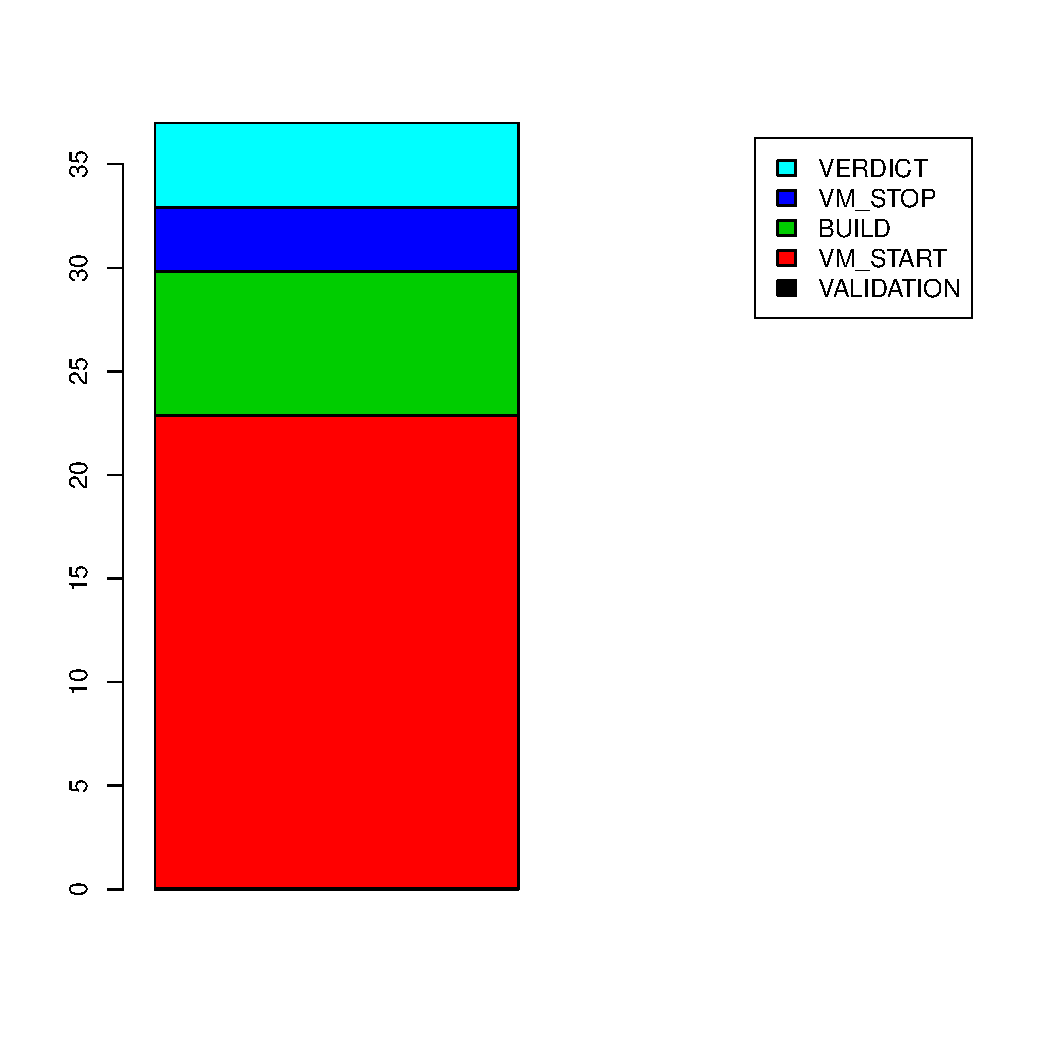
\includegraphics[width=70mm]{./libvirt_bar.pdf}
\end{frame}

% -- Более детальное аналогичное исследование, проведенное для этой
% -- самой медленной стадии показало следующее.
% -- Больше всего времени тратится на получение IP адреса виртуальной
% -- машиной. 
\begin{frame}{Профилирование}
	Парсинг логов \textit{pdaemon.sh}
	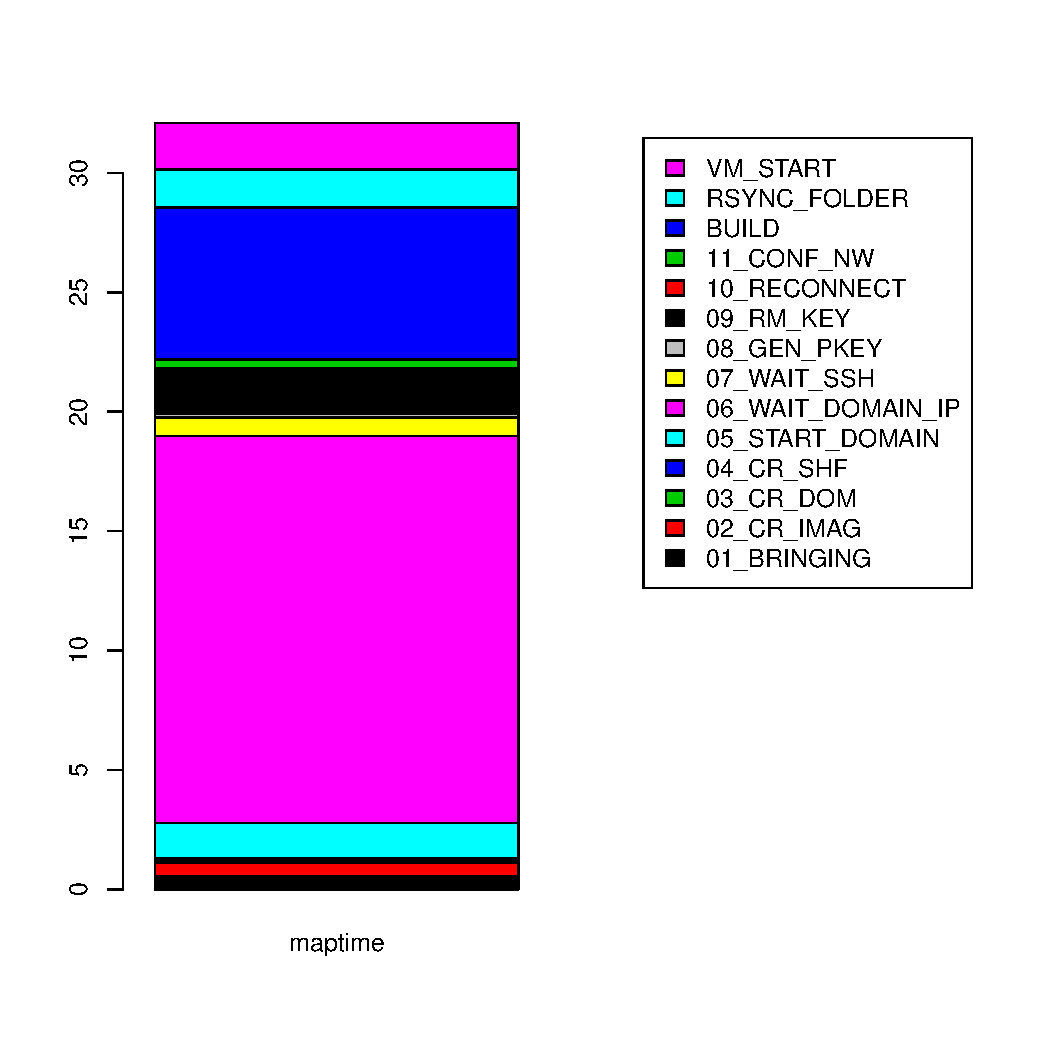
\includegraphics[width=70mm]{./vm_start_bar.pdf}
\end{frame}

% -- К сожалению, оказалось, что простое отключение DHCP-сервера в 
% -- настройках Vagrantfile не решает проблемы, и требуется более
% -- тонкое конфигурирование
\begin{frame}{Оптимизация по времени}
	\begin{itemize}
		\item Конфигурирование сетевых настроек загружаемого образа
		\item Создание постоянной конфигурации со статическим IP для Libvirt 
	\end{itemize}
\end{frame}

% -- В рамках этого проекта мне удалось поработать со следующими тех-
% -- нологиями (небольшое перечисление с коментариями по ходу)
\begin{frame}{Технологии}
	\begin{itemize}
		\item ОС (гостевая и хостовая): \textbf{GNU/Linux}
		\item Виртуализация: \textbf{QEMU/KVM}, \textbf{Vagrant} + (\textbf{Docker} || \textbf{Libvirt})
		\item Языки: \textbf{Ruby}, \textbf{Python}, \textbf{Bash}, \textbf{R}
		\item Система контроля версий: \textbf{Git}
		\item Удаленный доступ: \textbf{SSH}
		\item Коммуникация: \textbf{Slack}
	\end{itemize}
\end{frame}

% -- Резюмируя
\begin{frame}{Результаты}
	\begin{itemize}
		\item Проверяющая система отделена от тестовых сценариев
		\item Создание автоматических тестов производительности системы
		\item Ускорение проверки!
	\end{itemize}
\end{frame}

\begin{frame}{Перспективы}
	Проект не завершен в полной мере, ещё есть направления для развития:
	\begin{itemize}
		\item Интеграция изменений
		\item Автоматические тесты производительности могут быть совершеннее
		\item Дальнейший рефакторинг кода
		\item Потенциально возможно дальнейшее ускорение проверки
		\item Автоматизация конфигурирования оптимальных настроек 
	\end{itemize}
\end{frame}

% -- Ссылка на тот самый курс
\begin{frame}{Ссылки}
	\begin{itemize}
		\item Курс: \textbf{https://stepik.org/course/2051}
	\end{itemize}
\end{frame}

\begin{frame}{Emails}
	\begin{itemize}
		\item Волков Д. \textbf{volkov12@rambler.ru}
		\item Заславский М. \textbf{mark.zaslavskiy@gmail.com}
	\end{itemize}
\end{frame}

\begin{frame}{Ссылки}
	\begin{itemize}
		\item \textbf{https://github.com/OSLL/mooc-lp-optimization}
	\end{itemize}
\end{frame}

\end{document}
